% !TEX root = ../main.tex
\lecture{9}{2026-11-10}{Promotion/Kommunikation}
\textit{\textbf{siehe Folien:}} \url{https://lms.uzh.ch/auth/RepositoryEntry/17910989063/CourseNode/96531468745796/path%3D~~Vorlesung%204/0}
\subsection{Marketingprozess III: Marketingprogramm Promotion}
\subsubsection{Integrierte Kommunikation}

\begin{itemize}
    \item \textbf{Koordination und Integration} alle Botschaften sind einheitlich und über alle Kommunikationskanäle verteilt.
    \item \textbf{inhaltliche und formale Abstimmung} der Instrumente in der Kommunikation
    \item Ziel: klare einheitliche Botschaft über das unternehmen
    \item Voraussetzung: Alle Kontaktpunkte mit Kunden müssen bekannt sein
\end{itemize}

\subsubsection{Push-Pull-Strategie}

\begin{itemize}
    \item 3 Knoten (Hersteller, Einzel/Grosshandel, Endkonsument)
    \item \textbf{Push}
    \begin{itemize}
        \item Produkte werden ohne direkte Anfragen/Absprache mit Konsumente an den Markt gebracht.
    \end{itemize}
    \item \textbf{Pull}
    \begin{itemize}
        \item Waren werden produziert nach direkten Anfragen des Kunden. Personalisiert,
    \end{itemize}
\end{itemize}

\subsubsection{6 Stufen - Hierarchy of Effects}
\begin{itemize}
    \item Bewusstsein (Brandawareness)
    \begin{itemize}
        \item Bekanntheit
        \item Überhaupt wissen, das eine Marke existiert
    \end{itemize}
    \item Wissen
    \begin{itemize}
        \item Informationen über die Marke und Produkte sammeln
    \end{itemize}
    \item Sympathie
    \begin{itemize}
        \item Schaffung positiver Eindrücke
    \end{itemize}
    \item Präferenz
    \begin{itemize}
        \item Vorliebe für die Marke durch die Zielgruppe 
    \end{itemize}
    \item Überzeugung
    \begin{itemize}
        \item Die Marke ist besser als andere
    \end{itemize}
\end{itemize}

\begin{definition}
    [Aufmerksamkeit] Unbewusster Prozess der Auswahl gewisser Stimuli, die bewusst wahrgenommen werden sollen.
\end{definition}
\begin{definition}
    [Priming]
Um die Wahrnehmung des Konsumenten zu manipulieren/lenken können komplementäre Aspekte eines Produkts genutzt werden. Zum Beispiel französische Musik um die Wahl eines französischen Weins zu steigern.
Die Abrufbarkeit mentaler Schemata, Merkmalen können durch diese kurze Erfahrungen/Wahrnehmungen erhöht werden.
\end{definition}
\begin{definition}
    [Konditionierung]
Durch Wiederholung eines Stimulus und Nachfolgende Belohnung oder Ereignis, wird den Stimulus von Subjekt unmittelbar mit der Belohnung oder folgende Handlung verknüpft.
\end{definition}


\subsubsection{Werbung}
\begin{definition}
    [Werbung] alle bezahlte Formen nicht-persönlicher Präsentation einer Dienstleistung, Idee oder Produkt in Massenmedien.
\end{definition}

\textbf{Funktionen}
\begin{itemize}
    \item Informieren
    \begin{itemize}
        \item Bekanntheit schaffen
        \item Unrichtige Eindrücke korrigieren
    \end{itemize}
    \item Überzeugen
    \begin{itemize}
        \item Präferenz schaffen
        \item Wechsel aus andere Marken
        \item Zum Kauf animieren
    \end{itemize}
    \item Erinnern
    \begin{itemize}
        \item Ein Produkt könnte in naher Zukunft nötig sein
        \item Erinnern wo das Produkt zu finden ist
        \item Saisonale Produkte 
    \end{itemize}
\end{itemize}

\textbf{Budget Faktoren}
\begin{itemize}
    \item Phase des Produktlebenszyklus (Wenn Degeneration lohnt es sich nicht)
    \item Marktanteil des Produkts (Wenn schon gross, muss nicht viel investiert werden)
    \item Wettbewerbintensität
    \item Häufigkeit
    \item Produktdifferenzierung 
\end{itemize}
\pagebreak
\textbf{Budget Entscheidung}
\begin{itemize}
    \item All you can afford
    \item Als Prozentsatz des Umsatzes
    \item Im Vergleich zur Konkurrenz
    \begin{itemize}
        \item Game-Theory
    \end{itemize}
    \item Anhand Marketing Ziele und Aufgaben
\end{itemize}

\textbf{Werbe Formel AIDA}
\begin{itemize}
    \item Attention
    \item Interest
    \item Desire
    \item Action
\end{itemize}

\subsubsection{Public Relations}

\textbf{Aufgaben}
\begin{itemize}
    \item Wartung der Image des Unternehmens
    \item Kontakt zur Presse
    \item Lobbying 
    \item Veröffentlichung der Produkte
    \item Aufbau Investorenbeziehungen
\end{itemize}

\textbf{Instrumente}
\begin{itemize}
    \item Press Conference
    \item PR-Events
    \item Info-material
    \item Corporate
    \item Sponsoring
\end{itemize}

\subsection{Marketingprozess IV: Aufbau profitabler Kundenbeziehungen}

\subsubsection{CRM-Konzept}
\begin{itemize}
    \item Gesamtprozess Aufbau und Erhaltung Kundenbeziehungen
    \item Transformation Massenmarketing in segmentierten Marketing
    \item Unterstützt von Datenbanken, Software und Interaktive Medien
\end{itemize}

\textbf{Kundenlebenswert} \linebreak
Nach Profitabilität und Dauer der Beziehung.\linebreak
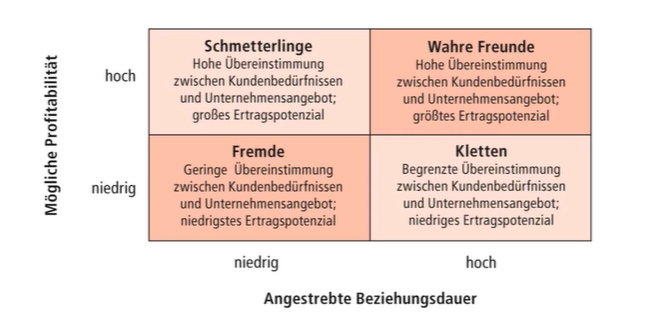
\includegraphics[width=\textwidth,height=0.7\textheight,keepaspectratio]{figures/Kundenlebenswert.png}
\subsubsection{Krisen}
Wie sollen Unternehmen in Krisen mit Kundschaft und Partner kommunizieren?
\begin{itemize}
    \item Opferkrise geringem Imageschaden (Stakeholder und Unternehmen benachteiligt)
    \begin{itemize}
        \item Denial von Verbindung des Unternehmens mit dem Ereignis
        
    \end{itemize}
    \item Unfallkrise mittlerem Schaden (Nicht absichtlich aber nur Kunden benachteiligt)
    \begin{itemize}
        \item Minderung der Schaden, Rechtfertigung des Problems
    \end{itemize}
    \item Vermeidbare Krise hohem Schaden (Unethische Absicht des Unternehmens )
    \begin{itemize}
        \item Übereinkunft: übernahme der Verantwortung, Entschuldigen, Besorgnis über Opfer
    \end{itemize}
\end{itemize}

\textbf{Wahrnehmungsfaktoren}

\begin{itemize}
    \item Krisenhistorie
    \item Andere negative Erfahrungen
\end{itemize}

\pagebreak
\subsection{Marketing IV: Vorlesung ON-Fallstudie}
 Wieso gingen Verkaufszahlen in der Schweiz zurück, während sie weltweit stiegen?
\subsubsection{Kommunikationsprozess}
\begin{enumerate}
    \item Sender
    \item Kodierung (Symbole, Sprache, Persönlichkeiten)
    \item Botschaft/Medium (Objektiver Ausdruck der Kodierung)
    \item Dekodierung (Interpretation der Zielgruppenmitglieder)
    \begin{itemize}
        \item Sehr oft lauft Marketing-Kommunikation in dieser Phase schief 
        \item Bestehe
    \end{itemize}
    \item Empfänger (Individuelle Personen)
\end{enumerate}

\begin{itemize}
    \item Bedeutung entsteht beim Empfänger
    \item Erfahrung der Sender und Empfänger müssen überlappen, um Missverständnisse zu vermeiden
\end{itemize}

\subsubsection{Hierarchy of effects}

\begin{itemize}
    \item Botschaft und Budget in den Phasen ansetzen (Bewusstsein, Wissen, usw.), wo die Zielgruppe stecken bleibt 
    \begin{itemize}
        \item Wenn Marke schon bekannt aber noch wenige die Wissensphase durchmachen, sollte mehr Ressourcen in dieser Phase investiert werden
    \end{itemize}
    \item Eigene Ziele und KPIs für jede Phase
    \begin{itemize}
        \item Umsatz misst Kauf und nicht Sympathie
    \end{itemize}
    \item Barrieren zwischen Phasen erkennen
    \begin{itemize}
        \item Preis zwischen Überzeugung und Kauf
    \end{itemize}
\end{itemize}

\subsubsection{Was ON Kodiert und was empfangen wird}
\begin{itemize}
    \item Kodierung
    \begin{itemize}
    \item Swiss-engineering 
    \item Premium Qualität hohe preise
    \item Roger Federer als Investor
    \item Celebrities (meist bei jüngeren Menschen bekannt)
\end{itemize}
\item Dekodierung (USA,ASIEn)
\begin{itemize}
    \item 1/3 der Kundschaft unter 34
\end{itemize}
\item Dekodierung (Schweiz)
\begin{itemize}
    \item Schuhe für Rentner/Eltern (Aus Umfeld)
    \item Fehldekodierung besteht im Erfahrungsfeld des Empfängers und nicht allein durch die Botschaft
\end{itemize}
\end{itemize}

\subsubsection{Dekodierung Kampagnen}

\begin{itemize}
    \item Elmo Soft Wins
    \begin{itemize}
        \item Botschaft Sympathie
        \begin{itemize}
            \item Jung, locker, unseriös
        \end{itemize} 
        \item Botschaft Wissen
        \begin{itemize}
            \item Geeignet fürs joggen/running 
            \item Soft -> Bequemlichkeit der Sohle
        \end{itemize}
        \item Pretest Fragen (Testen ob die Botschaft entsprechend dekodiert wurde)
        \begin{itemize}
            \item Vor einer Massenverteilung der Werbung sollte kleine Gruppe befragt werden
            \item Womit verknüpfen sie ON-Schuhe?
        \end{itemize}
    \end{itemize}
\end{itemize}

\subsubsection{Key Takeaways}

\begin{enumerate}
    \item Bedeutung steht beim Empfänger
    \item Efforts an der Phase setzen, an der potenzielle Kunden stecken bleiben
    \item Spezifische KPIs für jede Stufe  
    \item Pretesting der Botschaft mit standartisierten Fragen
    \item Erfolgskontrolle
\end{enumerate}


